\documentclass{article}
\usepackage{geometry}
\geometry{
  a4paper,
  margin=0.25in
}

\renewcommand\labelitemi{*}

% Packages
% ------------------
\usepackage{tkz-euclide}
\usepackage{tikz} % for drawing diagrams
\usepackage{bm} % bold mode
\usepackage{subfig}
\usepackage{graphicx}
%% \usepackage{amsfonts}
\usepackage{amssymb}
\usepackage{amsmath}
%% \usepackage{amsthm}
\usepackage{color}
\usepackage{algorithm}
\usepackage{algpseudocode}
\usepackage{dsfont}
\usepackage{forest}

% setup style of tikzlibrary elements
% ------------------------------------
\usetikzlibrary{patterns}
\usetikzlibrary{patterns.meta}
\usetikzlibrary{arrows}
\usetikzlibrary{quotes,angles}
\usetikzlibrary{positioning}
\usetikzlibrary{plotmarks}
\usetikzlibrary{math}
\usetikzlibrary{shapes.geometric, arrows}
\tikzstyle{block} = [rectangle, minimum width=2.5cm, minimum height=1cm, text centered, text width=2.7cm, draw=black, fill=white]
\tikzstyle{redblock} = [rectangle, thick, minimum width=2.5cm, minimum height=1cm, text centered, text width=2.7cm, draw=red, fill=white]
\tikzstyle{wideblock} = [rectangle, minimum width=2.5cm, minimum height=1cm, text centered, text width=5cm, draw=black, fill=white]
\tikzstyle{tallblock} = [rectangle, minimum width=1.9cm, minimum height=2cm, text centered, text width=1.9cm, draw=black, fill=white]
\tikzstyle{inputblock} = [rectangle, minimum width=1.7cm, minimum height=5cm, text centered, text width=1.7cm, draw=black, fill=white]
\tikzstyle{startstop} = [rectangle, rounded corners, minimum width=3cm, minimum height=1cm, text centered, draw=black, fill=white]
\tikzstyle{startstop_wide} = [rectangle, rounded corners, minimum width=6cm, minimum height=1cm, text centered, draw=black, fill=white]
\tikzstyle{io} = [trapezium, trapezium left angle=70, trapezium right angle=110, minimum width=3cm, minimum height=1cm, text centered, draw=black, fill=white]
\tikzstyle{process} = [rectangle, minimum width=4cm, minimum height=1cm, text centered, text width=4cm, draw=black, fill=white]
\tikzstyle{decision} = [diamond, minimum width=3cm, minimum height=1cm, text centered, draw=black, fill=white]
\tikzstyle{arrow} = [->,>=stealth] % can add "thick" to make it bold
\tikzset{radiation/.style={{decorate,decoration={expanding waves,angle=90,segment length=4pt}}}}

% \tikzdeclarepattern{
%   name=customdashed,
%   bounding box={(-0.5pt,-0.5pt) and (10*1,1pt)},
%   tile size={(10*1, 4pt)},
%   tile transformation={},
%   code={
%     % Dash lengths (in pt or any TeX length)
%     \draw[line width=0.4pt]
%     (0pt,0pt) -- (20pt,0pt)
%     (25pt,0pt) -- (38pt,0pt)
%     (43pt,0pt) -- (48pt,0pt)
%     (53pt,0pt) -- (85pt,0pt)
%     (90pt,0pt) -- (100pt,0pt);
%   }
% }

%% new commands
% ------------------
\newcommand{\fixme}{\textcolor{red}{\textbf{fix me}} \space}
\newcommand{\attention}[1]{\noindent \fixme \textcolor{red}{#1}}

% \definecolor{light-gray}{gray}{0.95}
% \newcommand{\code}[1]{\colorbox{light-gray}{\texttt{#1}}}


\begin{document}

% @@@@@@@@@@@@@@@@@@@@@@@@@@@@@@@@@@@@@@@@@@@@@@@@@@

\begin{figure}[h]
\begin{center}
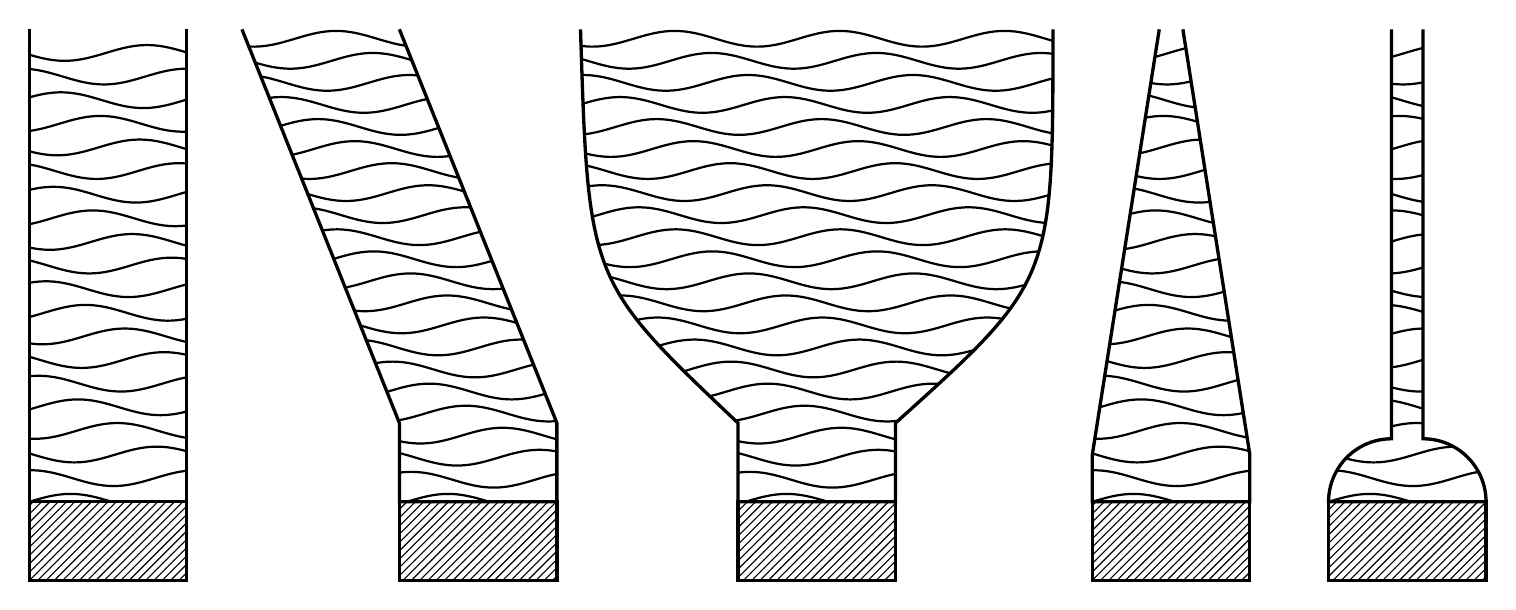
\begin{tikzpicture}[auto, node distance=2.7cm, >=latex']

  % % comment out
  % \draw[step=1cm,gray,very thin] (0,0) grid (20,\ymax);

  \tikzmath{\ymax = 7; \bh = 1; \width = 2;}

  % Fig 1
  \begin{scope}
    \draw[very thick] (0,0) rectangle +(\width,\bh);
    \draw[pattern={north east lines}] (0,0) rectangle +(\width,\bh);

    \draw[very thick] (0,\ymax) -- (0,\bh) -- (\width,\bh) -- (\width,\ymax);
    \clip (0,\ymax) -- (0,\bh) -- (\width,\bh) -- (\width,\ymax);

    \foreach \y in {0, 0.3, ..., 6} {
      \draw[thick]
      plot[domain=0:\width, smooth, samples=50]
      (\x, {\bh + sin(3*\x r + \y*5 r)*0.1 + \y});
    }
  \end{scope}

  % Fig 2
  \begin{scope}[xshift=2.7cm]
    \draw[very thick] (\width,0) rectangle +(\width,\bh);
    \draw[pattern={north east lines}] (\width,0) rectangle +(\width,\bh);

    \draw[very thick] (0,\ymax) -- (\width,\bh*2) -- (\width,\bh) -- (\width*2,\bh) -- (\width*2,\bh*2) -- (\width,\ymax);
    \clip (0,\ymax) -- (\width,\bh*2) -- (\width,\bh) -- (\width*2,\bh) -- (\width*2,\bh*2) -- (\width,\ymax);

    \foreach \y in {0, 0.28, ..., \ymax} {
      \draw[thick]
      plot[domain=0:\width*2, smooth, samples=50]
      (\x, {1+sin(3*(\x) r + \y*5 r)*0.1 + \y});
    }
  \end{scope}

  % Fig 3
  \begin{scope}[xshift=7cm]
    \tikzmath{\c = 0.7; \cy1 = (\ymax + \bh*2) / 2 - \c;}

    \draw[very thick] (\width,0) rectangle +(\width,\bh);
    \draw[pattern={north east lines}] (\width,0) rectangle +(\width,\bh);

    \draw[very thick] (0,\ymax) .. controls (0.1,\cy1) .. (\width,\bh*2) -- (\width,\bh) -- (\width*2,\bh) -- (\width*2,\bh*2) .. controls (\width*3,\cy1) .. (\width*3,\ymax);
    \clip (0,\ymax) .. controls (0.1,\cy1) .. (\width,\bh*2) -- (\width,\bh) -- (\width*2,\bh) -- (\width*2,\bh*2) .. controls (\width*3,\cy1) .. (\width*3,\ymax);

    \foreach \y in {0, 0.28, ..., \ymax} {
      \draw[thick]
      plot[domain=0:\width*3, smooth, samples=50]
      (\x, {1+sin(3*(\x) r + \y*5 r)*0.1 + \y});
    }
  \end{scope}

  % Fig 4
  \begin{scope}[xshift=13.5cm]
    \tikzmath{\m = 1.6; \d = 0.15;}

    \draw[very thick] (0,0) rectangle +(\width,\bh);
    \draw[pattern={north east lines}] (0,0) rectangle +(\width,\bh);

    \draw[very thick] (\width/2-\d,\ymax) -- (0,\bh*\m) -- (0,\bh) -- (\width,\bh) -- (\width,\bh*\m) -- (\width/2+\d,\ymax);

    \clip (\width/2-\d,\ymax) -- (0,\bh*\m) -- (0,\bh) -- (\width,\bh) -- (\width,\bh*\m) -- (\width/2+\d,\ymax);

    \foreach \y in {0, 0.3, ..., \ymax} {
      \draw[thick]
      plot[domain=0:\width, smooth, samples=50]
      (\x, {1+sin(3*(\x) r + \y*5 r)*0.1 + \y});
    }
  \end{scope}

  % Fig 5
  \begin{scope}[xshift=16.5cm]
    \tikzmath{\d = 0.2; \yd = 1.8;}

    \draw[very thick] (0,0) rectangle +(\width,\bh);
    \draw[pattern={north east lines}] (0,0) rectangle +(\width,\bh);

    \draw[very thick] (\width/2-\d,\ymax) -- (\width/2-\d,\bh*\yd) arc (90 : 180 : 0.8cm) -- (\width,\bh) arc (0 : 90 : 0.8cm) -- (\width/2+\d,\ymax);
    \clip (\width/2-\d,\ymax) -- (\width/2-\d,\bh*\yd) arc (90 : 180 : 0.8cm) -- (\width,\bh) arc (0 : 90 : 0.8cm) -- (\width/2+\d,\ymax);

    \foreach \y in {0, 0.3, ..., \ymax} {
      \draw[thick]
      plot[domain=0:\width, smooth, samples=50]
      (\x, {1+sin(3*(\x) r + \y*5 r)*0.1 + \y});
    }
  \end{scope}


\end{tikzpicture}
\end{center}
 \caption{Duhem-1905N,fig-1}
\label{fig:Duhem-fig1}
\end{figure}

% @@@@@@@@@@@@@@@@@@@@@@@@@@@@@@@@@@@@@@@@@@@@@@@@@@


\begin{figure}[h]
\begin{center}
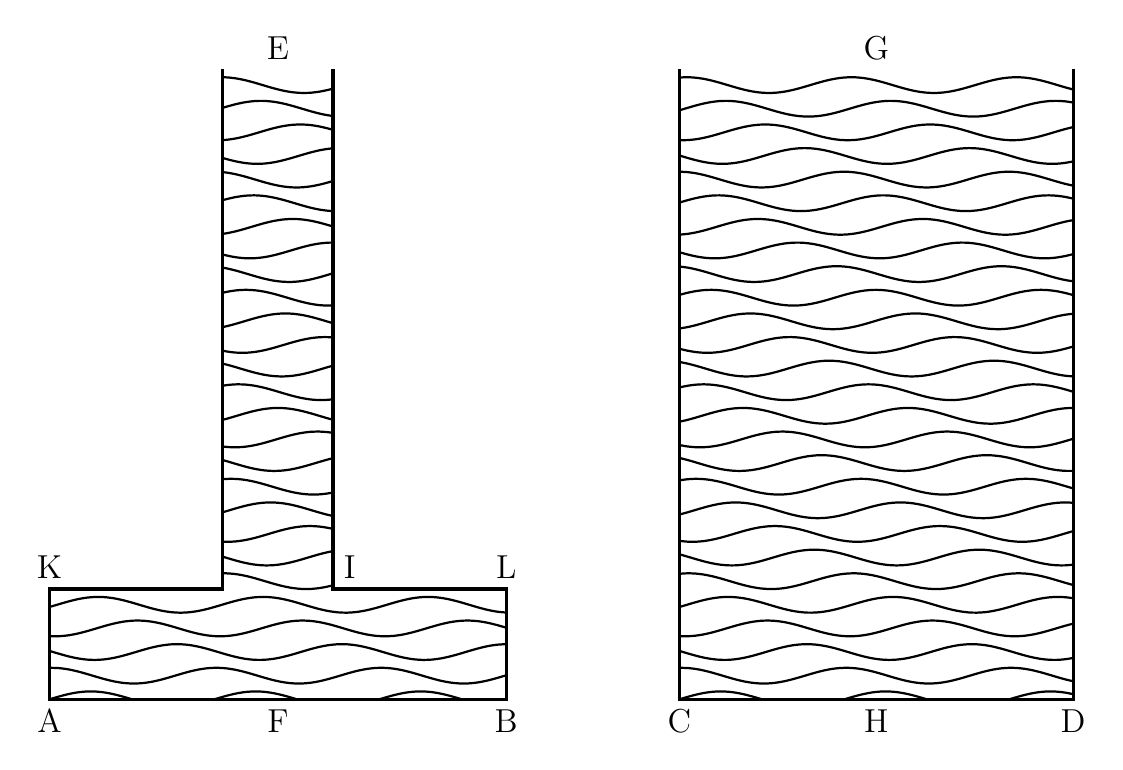
\begin{tikzpicture}[auto, node distance=2.7cm, >=latex']

  \tikzmath{\ymax = 8;}

  % Fig 1
  \begin{scope}
    \tikzmath{\w = 2.2; \h = 1.4; \tw = 1.4;}
    \tikzmath{\maxw = 2*\w+\tw;}

    \draw (\maxw/2,\ymax) node[above]{\large E};

    \draw[very thick] (\w,\ymax) -- (\w,\h) -- (0,\h) node[above]{\large K} -- (0,0) node[below]{\large A} -- node[below]{\large F} (\maxw,0) node[below]{\large B} -- (\maxw,\h) node[above]{\large L} -- (\w+\tw,\h) node[above right]{\large I} -- (\w+\tw,\ymax);

    \clip (\w,\ymax) -- (\w,\h) -- (0,\h) -- (0,0) -- (\maxw,0) -- (\maxw,\h) -- (\w+\tw,\h) -- (\w+\tw,\ymax);

    \foreach \y in {0, 0.3, ..., \ymax} {
      \draw[thick]
      plot[domain=0:\maxw, smooth, samples=50]
      (\x, {sin(3*\x r + \y*5 r)*0.1 + \y});
    }
  \end{scope}

  % Fig 2
  \begin{scope}[xshift=8cm]
    \tikzmath{\width = 5;}

    \draw (\width/2,\ymax) node[above]{\large G};
    \draw[very thick] (0,\ymax) -- (0,0) node[below]{\large C} -- node[below]{\large H} (\width,0) node[below]{\large D} -- (\width,\ymax);

    \clip (0,\ymax) -- (0,0) -- (\width,0) -- (\width,\ymax);

    \foreach \y in {0, 0.3, ..., \ymax} {
      \draw[thick]
      plot[domain=0:\width, smooth, samples=50]
      (\x, {sin(3*\x r + \y*5 r)*0.1 + \y});
    }
  \end{scope}

\end{tikzpicture}
\end{center}
 \caption{Duhem-1905N,fig-2}
\label{fig:Duhem-fig2}
\end{figure}


% @@@@@@@@@@@@@@@@@@@@@@@@@@@@@@@@@@@@@@@@@@@@@@@@@@


\begin{figure}[h]
\begin{center}
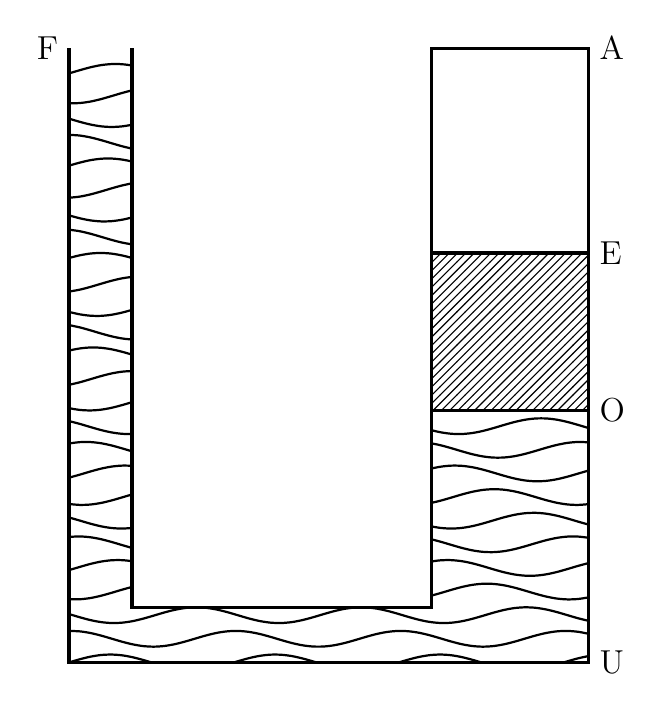
\begin{tikzpicture}[auto, node distance=2.7cm, >=latex']

  \tikzmath{\ymax = 7.8; \w1 = 0.8; \w2 = 3.8; \w3 = 2; \bh = 0.7;}
  \tikzmath{\o = 3.2; \e = \o + \w3;}
  \tikzmath{\width = \w1 + \w2 + \w3;}

  \draw[very thick] (\w1+\w2,\e) rectangle +(\w3,\ymax-\e) node[right]{\large A};
  \draw[very thick] (\w1+\w2,\o) rectangle +(\w3,\w3) node[right]{\large E};
  \draw[pattern={north east lines}] (\w1+\w2,\o) rectangle +(\w3,\w3);

  \draw[very thick] (0,\ymax) node[left]{\large F} -- (0,0) -- (\w1+\w2+\w3,0) node[right]{\large U} -- (\w1+\w2+\w3,\o) node[right]{\large O} -- (\w1+\w2,\o) -- (\w1+\w2,\bh) -- (\w1,\bh) -- (\w1,\ymax);

  \clip (0,\ymax) -- (0,0) -- (\w1+\w2+\w3,0) -- (\w1+\w2+\w3,\o) -- (\w1+\w2,\o) -- (\w1+\w2,\bh) -- (\w1,\bh) -- (\w1,\ymax);

  \foreach \y in {0, 0.3, ..., \ymax} {
    \draw[thick]
    plot[domain=0:\width, smooth, samples=50]
    (\x, {sin(3*\x r + \y*5 r)*0.1 + \y});
  }

\end{tikzpicture}
\end{center}
 \caption{Duhem-1905N,fig-3}
\label{fig:Duhem-fig3}
\end{figure}

% @@@@@@@@@@@@@@@@@@@@@@@@@@@@@@@@@@@@@@@@@@@@@@@@@@

\begin{figure}[h]
\begin{center}
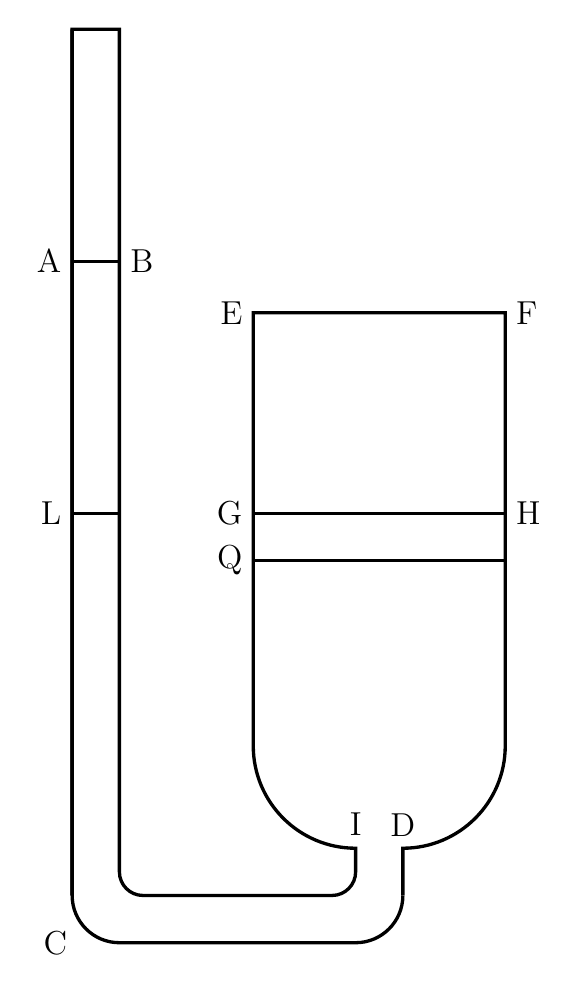
\begin{tikzpicture}[auto, node distance=2.7cm, >=latex']

  \tikzmath{\ymax = 11.6; \b = 0.6; \xmax = 3.6; \th = 5.5;}
  \tikzmath{\lt = \xmax;}
  \tikzmath{\rt = \xmax;}
  \tikzmath{\r1 = \b; \r2 = 1.3; \r3 = 0.3;}

  % % comment out
  % \draw[step=1cm,gray,very thin] (0,0) grid (\xmax*2,\ymax);

  \draw[very thick] (0,\ymax) -- (0,\b) arc (180 : 270 : \r1) node[left, xshift=-1.5em]{\large C} -- (\rt,\b-\r1) arc (270 : 360 : \r1);
  \draw[very thick] (\rt+\r1,\b) -- node[above, yshift=0.9em]{\large D} (\rt+\r1,\r1+\b) arc (270 : 360 : \r2) -- (\rt+\r1+\r2,\r1+\b+\r2+\th) node[right]{\large F} -- (\lt-\r2,\r1+\b+\r2+\th) node[left]{\large E} -- (\lt-\r2,\r1+\r2+\b) arc(180 : 270 : \r2) node[above, yshift=0.08em]{\large I} -- (\lt,\b+\r3) arc(360 : 270 : \r3);
  \draw[very thick] (\lt-\r3,\b) -- (\b+\r3,\b) arc (270 : 180 : \r3) -- (\b,\ymax) -- (0,\ymax) -- (0,\b);
  \tikzmath{\tw = \r1+2*\r2;}

  % Two horizontal lines
  \tikzmath{\p = 1.5;}
  \draw[very thick] (\lt-\r2,\r1+\th/2+\p) node[left]{\large Q} -- (\lt+\b+\r2,\r1+\th/2+\p);
  \draw[very thick] (\lt-\r2,\r1+\th/2+\b+\p) node[left]{\large G} -- (\lt+\b+\r2,\r1+\th/2+\p+\b) node[right]{\large H};

  \draw[very thick] (0,\r1+\th/2+\p+\b) node[left]{\large L} -- (\b,\r1+\th/2+\p+\b);
  \draw[very thick] (0,\r1+\th/2+\p+\b+\tw) node[left]{\large A} -- (\b,\r1+\th/2+\p+\b+\tw) node[right]{\large B};

\end{tikzpicture}
\end{center}
 \caption{Duhem-1905N,fig-4}
\label{fig:Duhem-fig4}
\end{figure}


% @@@@@@@@@@@@@@@@@@@@@@@@@@@@@@@@@@@@@@@@@@@@@@@@@@



% -----------------------------
%% \bibliography{references}


% -----------------------------
\end{document}

%%% Local Variables:
%%% mode: latex
%%% TeX-master: t
%%% End:
